\section{Pré-étude} \label{sec:Pre-Etude}

\subsection{Fonctionnement du système} \label{ssec:Fonctionnement}
Le microcontrôleur interagît avec 4 périphériques principaux : Avec le \gls{GNSS}, il partage une communication qui lui permet d'obtenir les informations de localisation par le biais de plusieurs systèmes de satellites. Il y a ensuite, la centrale inertielle qui lui donne accès de une multitude de mesures sur 9 axes, or, ici les mesures gyroscopiques et d'accélération sont exploitées. La carte SD, permet quant-à-elle, de stocker toutes ces données pour avoir minimum les information des 15 dernières minutes de vol. Le dernier périphériques principale \gls{FTDI}, permet d'avoir une interface avec un ordinateur via connexion USB-C.

\subsection{Schéma bloc} \label{ssec:Schema-bloc}

\begin{figure}[h]
	\centering
	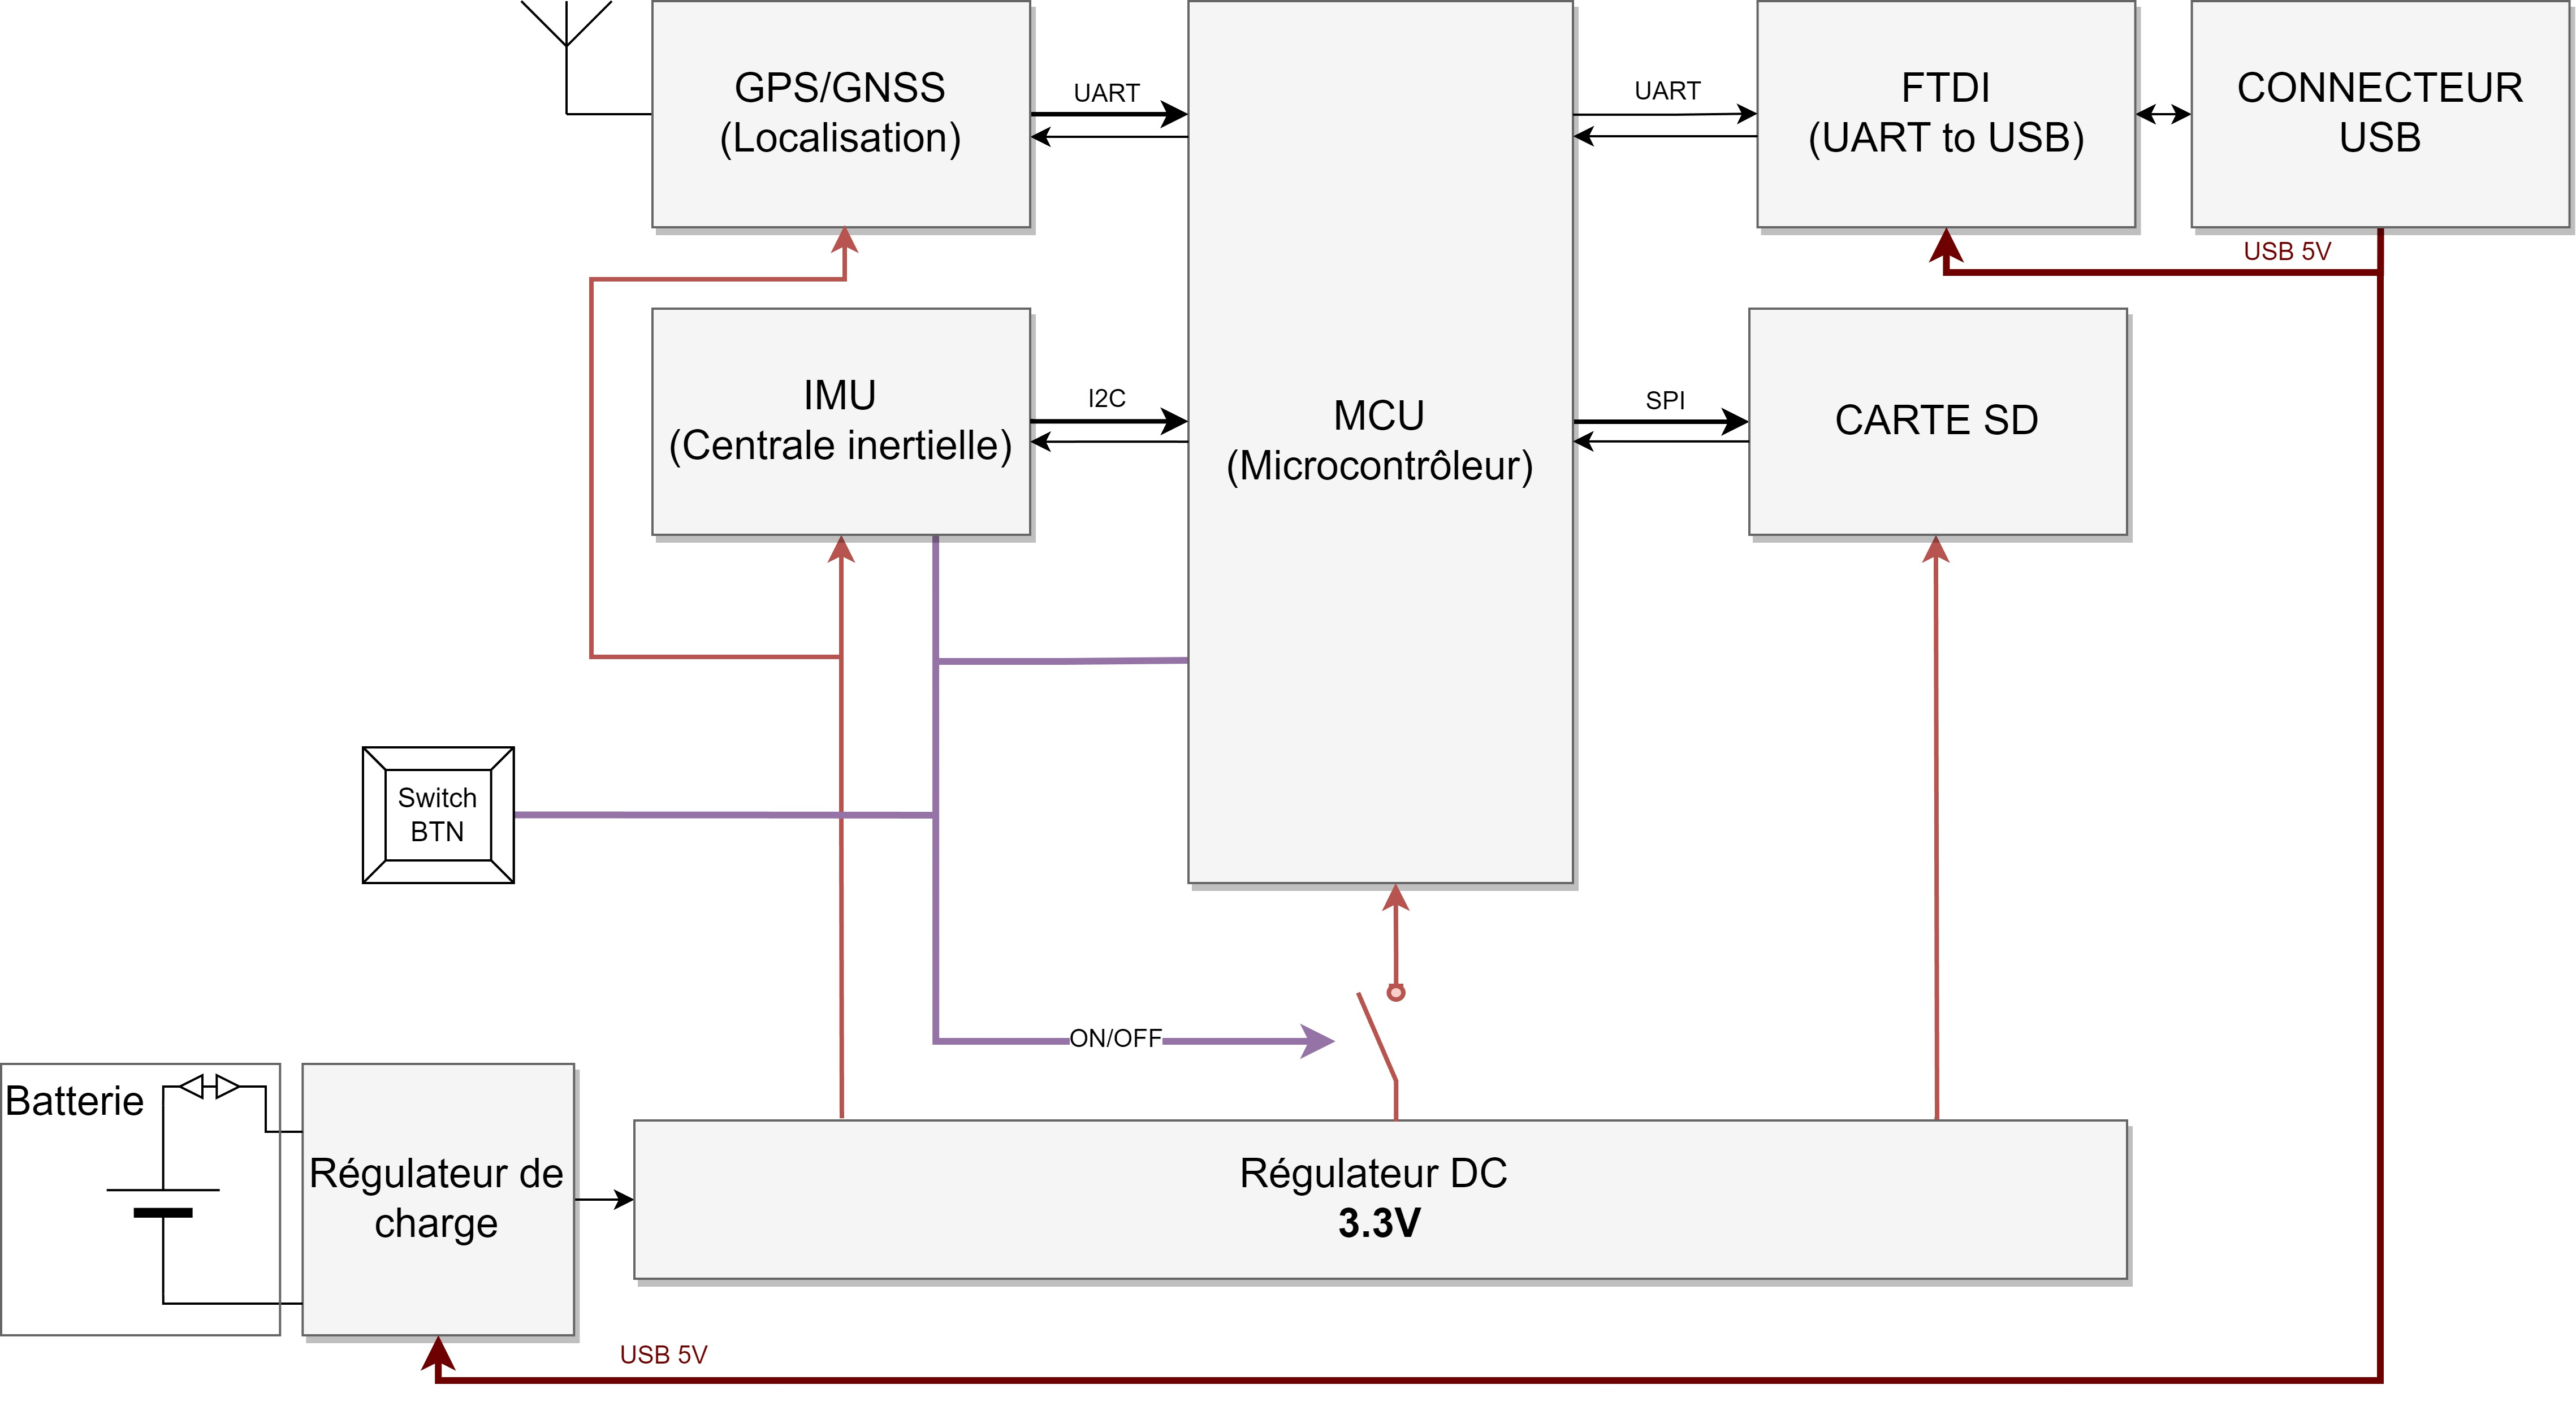
\includegraphics[width=1\textwidth]{../figures/cdc/blocs_grossiers_no_antenna.jpg}
	\caption{Schéma bloc}
	\label{fig:schbloc}
	\source{Auteur}
\end{figure}
% ---- Description des blocs ----
\subsection{Description des blocs} \label{ssec:Desc-blocs}

\begin{table}[h]
	\resizebox{\columnwidth}{!}{%
		\begin{tabular}{|l|l|}
			\hline
			Bloc         & Description                                                                         \\ \hline
			\Gls{gnss}.  & Récepteur \Gls{rf} avec antenne interne/externe et communication UART.              \\ \hline
			\Gls{mcu}.   & Microcontrôleur PIC32, intelligence du système, basse consommation.                 \\ \hline
			\Gls{imu}.   & Centrale inertielle, accélération, gyroscope...                                     \\ \hline
			Carte SD     & Stockage des données de vol.                                                        \\ \hline
			\Gls{FTDI}.  & Convertis la communication USB en série.                                            \\ \hline
			Régulateurs. & Le régulateur de charge gère la charge de l'accu. et un régulateur 3.3V le suit.    \\ \hline
			Batterie.    & La batterie est un accu que l'on peut charger par USB et permet une bonne autonomie. \\ \hline
		\end{tabular}%
	}
\end{table}

\clearpage
\raggedbottom
\subsection{Choix des composants et technologies} \label{sssec:ComposantsTech}
L'objectif de la pré-étude consiste en grande partie à sélectionner méthodiquement les technologies et les composants du projet. Cette partie du travail est essentielle et critique.

\paragraph{Microcontrôleur}
Le microcontrôleur nécessite au minimum les périphériques suivants : \\
\fbox{2 UART} \fbox{1 SPI} \fbox{1 I2C} \\
Il est préférable que le \gls{mcu} dispose de différentes configurations de gestion de puissance, notamment des modes d'économie d'énergie, afin d'avoir une maîtrise de la consommation et de permettre une meilleure autonomie. Enfin, le standard de l'école veut que les familles de microcontrôleurs PIC32 (Microchip) sont préférées.

\begin{figure}[h]
	\centering
	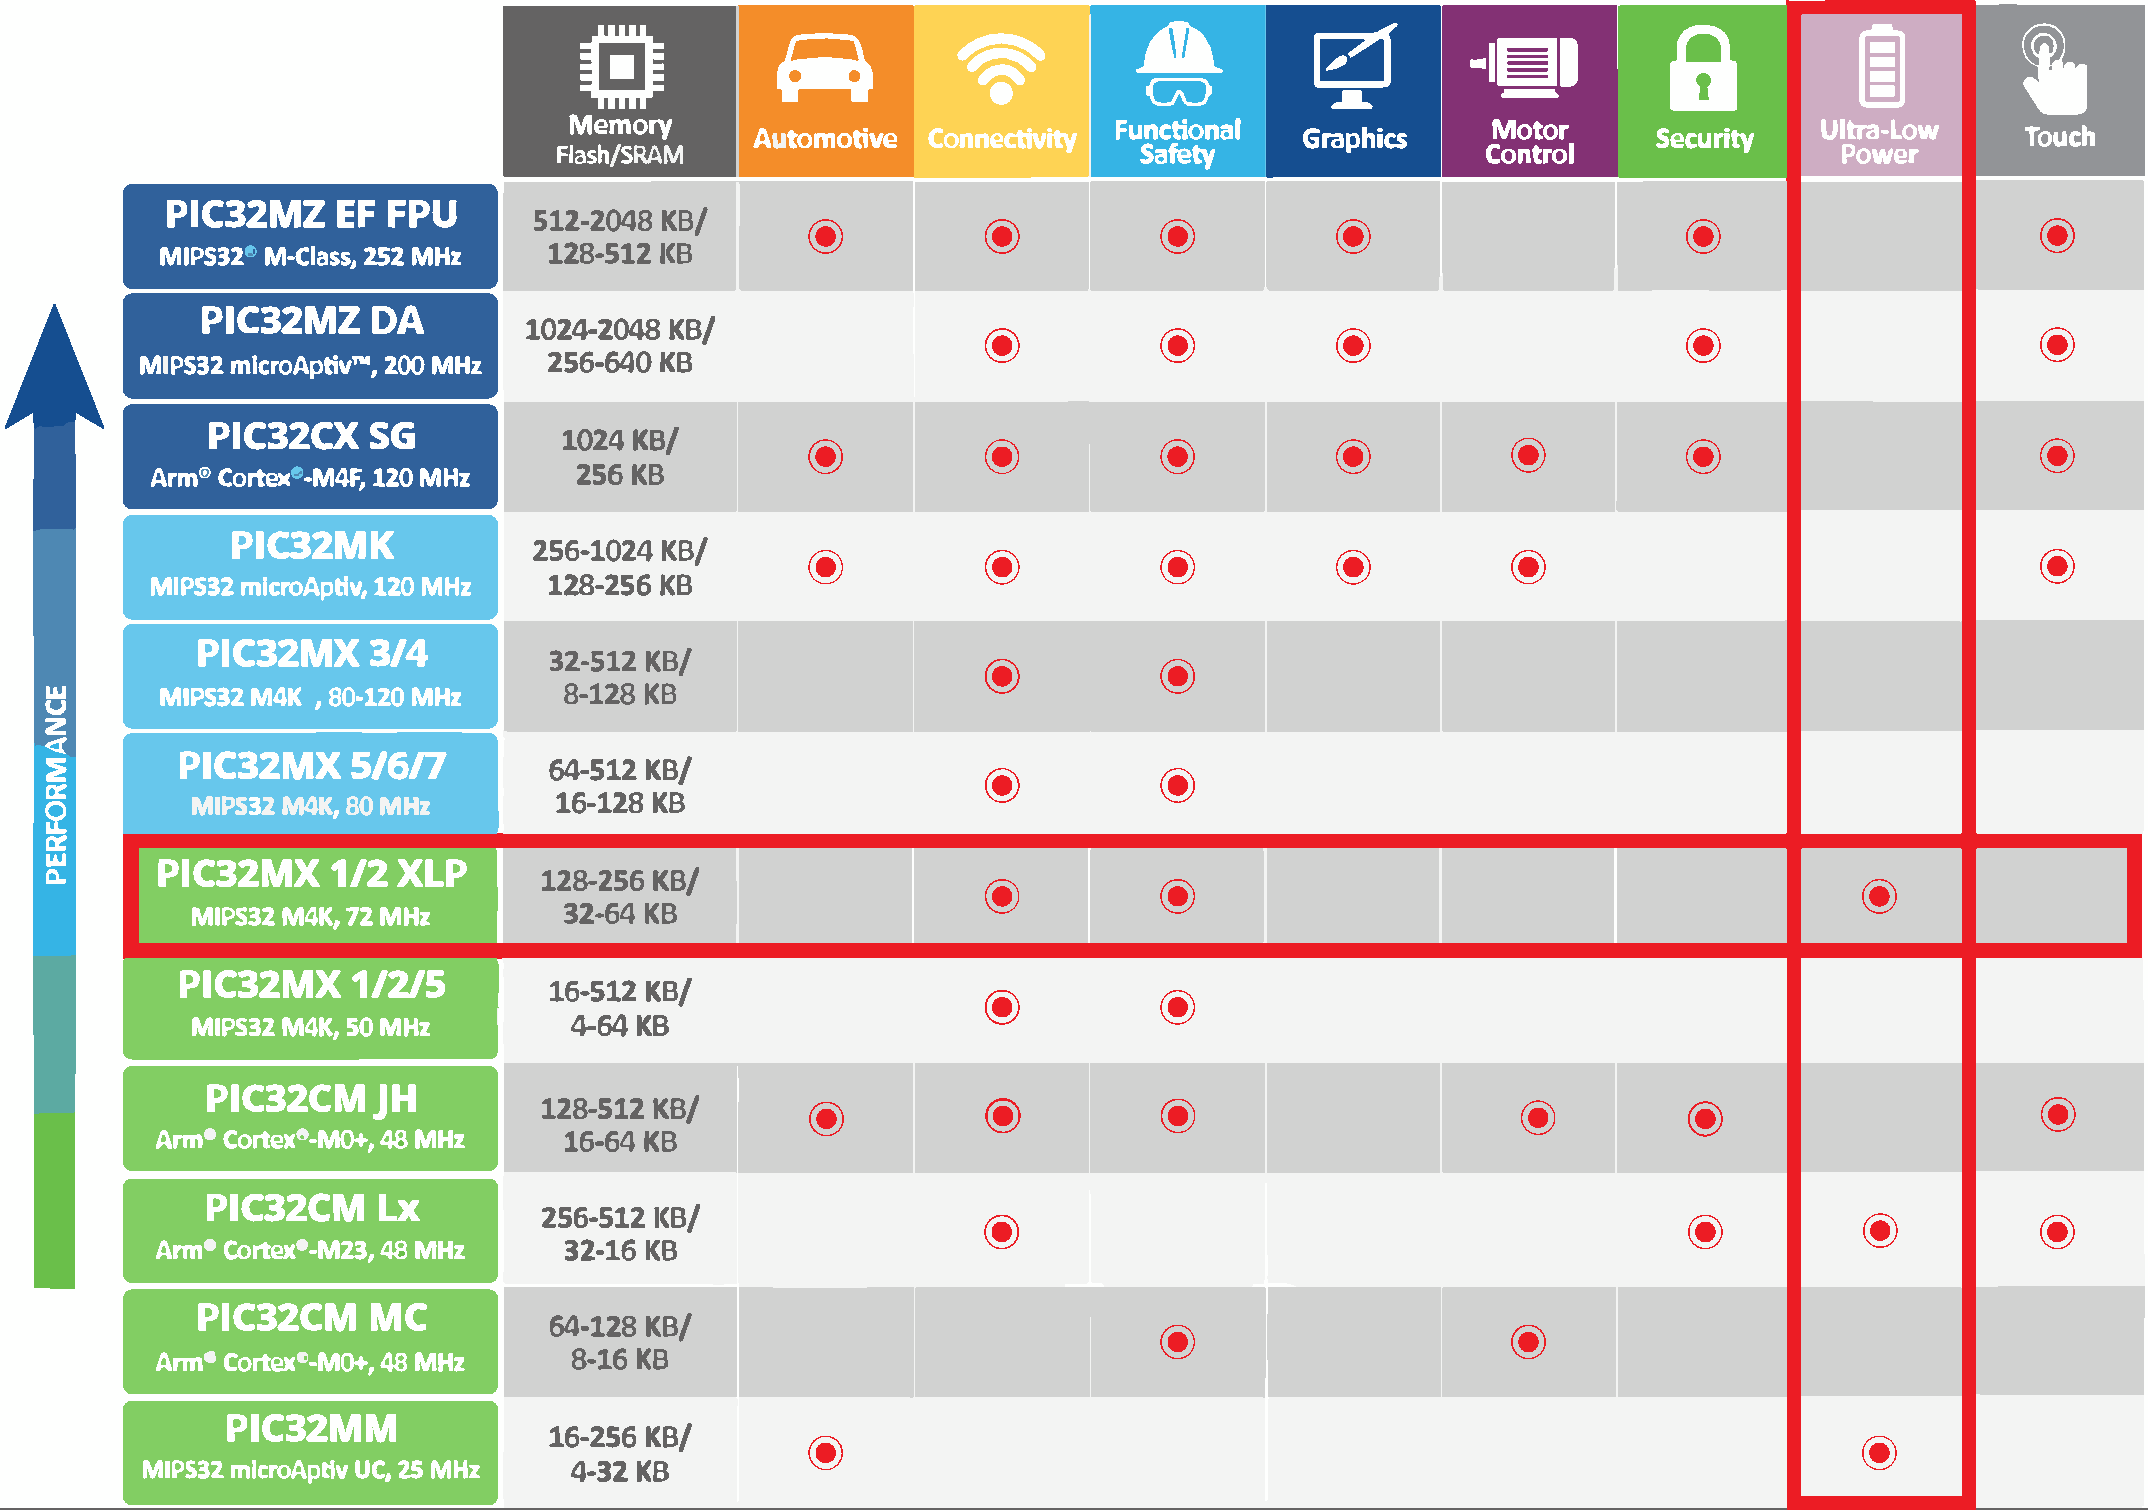
\includegraphics[width=0.7\linewidth]{../figures/pre_etude/familles_pic32}
	\caption{Familles PIC32}
	\label{fig:famillespic32}
	\source{\href{https://www.microchip.com/en-us/products/microcontrollers-and-microprocessors/32-bit-mcus/pic32-32-bit-mcus}{https://www.microchip.com/en-us/products/microcontrollers-and-microprocessors/32-bit-mcus/pic32-32-bit-mcus}}
\end{figure}

Sur la figure \ref{fig:famillespic32} le \gls{mcu} sélectionné appartient à la gamme 

\paragraph{Centrale inertielle} 
AAAAAA

\paragraph{GPS / GNSS}
AAAAA

\paragraph{Batterie, charge et régulation} 

\subsection{Systèmes d'économies d'énergie} \label{ssec:Low-power}
Dans le but de maximiser le temps de logging, des mécanismes d'économies d'énergie doivent être mis en place. 

\subsection{Estimation des coûts} \label{ssec:Estimation-Couts}
